\section{Text Creation} \label{textCreation}
By the time You start using this template, You have likely completed its contents using a more comfortable and collaborative software like Google Docs. Starting formatting makes sense only when the contents of Your work no longer change much. Otherwise, the changes in the content may require doing the formatting part again. Still, some formatting-related recommendations are relevant a lot earlier than when formatting the draft to a fair copy.

\subsection{Chapters}
Your thesis chapters should be evenly balanced with each other. Because this template focuses on formatting, then that guideline is broken here (the previous chapter~\ref{formatting} is noticeably lengthier than this chapter~\ref{textCreation}). In Your work, all the chapters besides the Introduction and Conclusion should have a relatively even length. This principle also helps You not overdo a single part of Your work but spread Your attention to all the essential parts. What precisely these parts are depends on Your thesis type. The University of Tartu’s Institute of Computer Science’s thesis preparation and grading guidelines document defines a certain number of these types. The study or research group where You are doing Your thesis might define continuations of those types. Ensure that Your thesis document provides a balanced coverage of all Your chosen thesis type requires.

\begin{wrapfigure}{r}{0.33\textwidth}
    \centering
    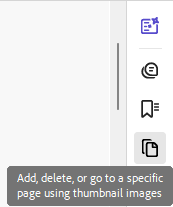
\includegraphics[width=0.33\textwidth]{figures/Figure5-AcrobatReaderMenu.png}
    \caption{The right-hand menu of Acrobat Reader.}
    \label{fig:acrobatReaderMenu}
\end{wrapfigure}
By the time Your thesis starts to take shape, it is useful to look at Your document as a whole. This can be done, for example, with the page order changing tool (\emph{Add, delete, or go to specific page using thumbnail images}) in the Acrobat Reader PDF viewer. The view from that tool shows You Your thesis as a whole. Just like if You would have printed out all of the pages and spread them across a desk. From that view, You see if all the different parts of the document are balanced and in visual equilibrium (see Figure~\ref{fig:acrobatReaderOverview}).

Seda saab teha näiteks Acrobat Reader PDF vaaturis lehekülgede järjekorra muutmise (\emph{Add, delete, or go to specific page using thumbnail images}) tööriistaga (vt joonis~\ref{fig:acrobatReaderMenu}). Tolle tööriista kuva näitab Teile tervet Teie tööd ülevaatlikult. Justkui oleksite oma töö välja printinud ja kõik lehed eraldi suure laua peale laotanud. Sellest ülevaatest Te näete, kas Teie erinevad töö osad on omavahel tasakaalus ja visuaalselt kooskõlas (vt joonis~\ref{fig:acrobatReaderOverview}).

\begin{figure}[t]
    \centering
    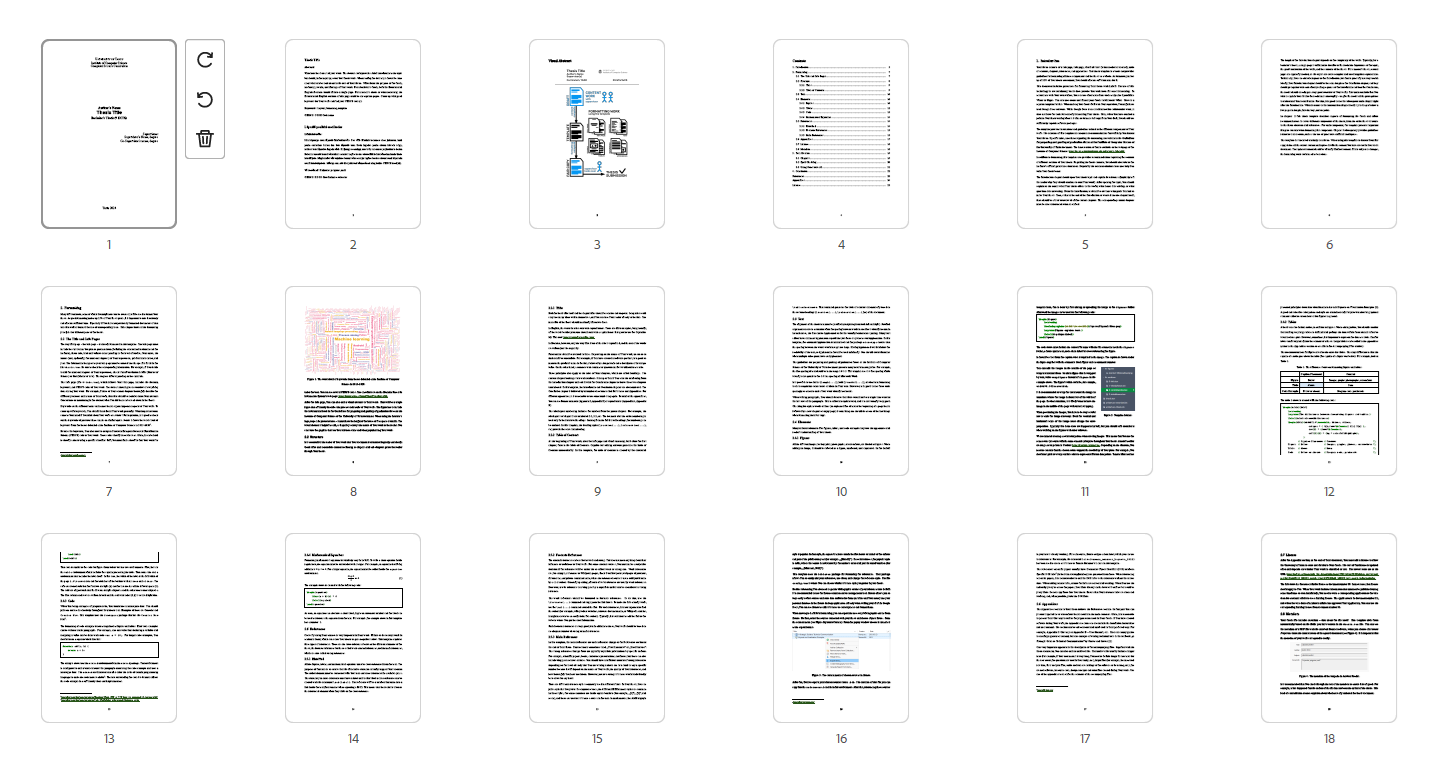
\includegraphics[width=\textwidth]{figures/Figure6-AcrobatReaderOverview.png}
    \caption{The overview of the thesis template in Acrobat Reader.}
    \label{fig:acrobatReaderOverview}
\end{figure}
he birds-eye view of the thesis also shows You if all the necessary places have text. For example, every chapter should start with a brief introductory text. This text must be after the   heading and before any subheadings. That introductory text usually explains why the corresponding chapter is necessary for Your work and what the reader can expect from the subchapters. In addition to that, the (sub)chapters could be woven together with connective sentences, and every bigger chapter could end with a conclusive paragraph. No chapter should start or end with any elements (figures, tables, code examples, equations) or a list. Your thesis text must be smooth to read.

\subsection{Spell Checking}
Microsoft Word’s speller, which You should turn on, comes in really handy when formatting Your fair copy. Having worked on Your draft a lot, You might have gotten used to looking at the same text over and over again; thus, noticing spelling mistakes Yourself might be quite difficult. There are spelling and proofing tools in Word for both the Estonian and English languages. Presenting a thesis that has grammatical errors can result in a lower grade.

Of course, You are also free to use tools that provide grammatical assistance, such as Grammarly, if You have access to such tools, and they make Your work more effective.

\subsection{Using Generative AI}
Using generative AI tools can also make Your work more effective. Here, their use for purely text editing purposes is focused on. When You have also used generative AI for content-related purposes (for example, to create Your questionnaire questions), You should definitely detail Your generative AI usage within the contents of Your thesis text. However, using it for editing Your thesis text is not content-related, so it will suffice to mention its use at the end of the Introduction chapter.

One good way to use a generative AI chatbot is to give it a paragraph of Your text and a prompt to make the specified academic text more readable. When doing that, You should read the result and correct it as needed. The AI chatbot might have mutated Your thoughts in the text, and You must restore them. Also, You might not personally agree with the specific style that AI has provided You and may want to keep tweaking it. The generative AI tools can very effectively help improve Your text flow, but You have to be very keen to ensure that the modified text still conveys Your thoughts and that You agree with the proposed writing style.

It is certainly not effective to use paragraphs that are solely generated by AI in Your thesis text. The author of the thesis is still You. This means that You are responsible for what is written in Your document. Typically, the text written by AI tends to be too general, overly illustrative and includes factual errors that a knowledgeable human author would not make. You do not want to put Yourself into a situation where You have to direct blame towards an AI chatbot due to issues in Your thesis text.
